\documentclass{standalone}
\usepackage{tikz}
\usetikzlibrary{patterns, positioning}


\begin{document}
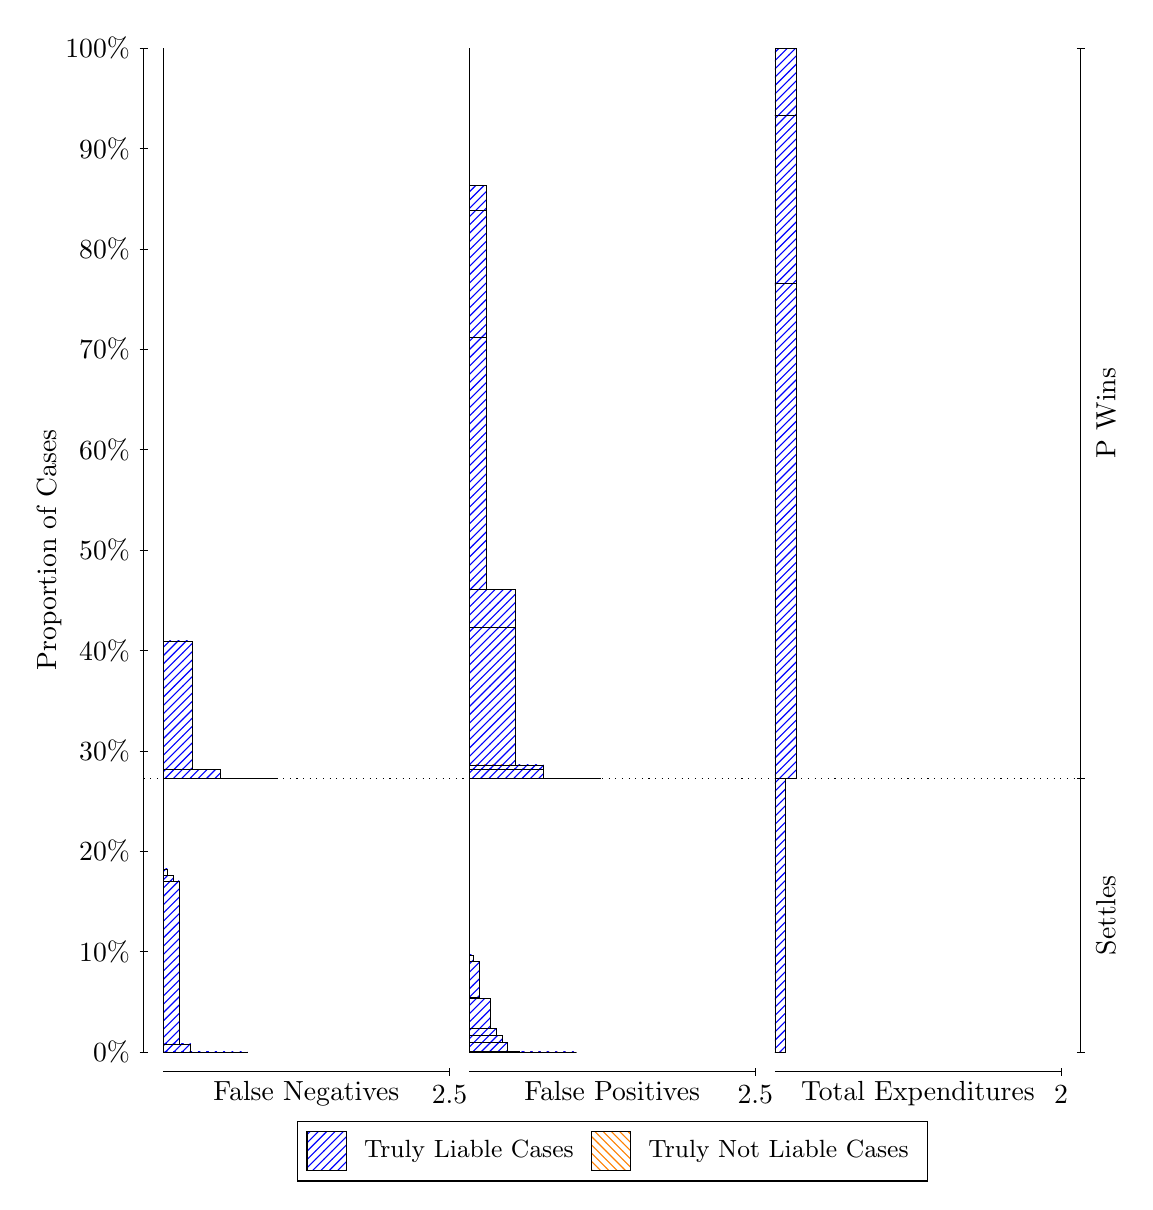
\begin{tikzpicture}
\draw[black, very thin] (1.5,1.75) -- (1.5,14.5);
\node[rotate=90, text=black, anchor=center] at (0.3, 8.125) {Proportion of Cases};
\draw[black, very thin] (1.45,1.75) -- (1.55,1.75);
\node[text=black, anchor=east] at (1.45, 1.75) {0\%};
\draw[black, very thin] (1.45,3.025) -- (1.55,3.025);
\node[text=black, anchor=east] at (1.45, 3.025) {10\%};
\draw[black, very thin] (1.45,4.3) -- (1.55,4.3);
\node[text=black, anchor=east] at (1.45, 4.3) {20\%};
\draw[black, very thin] (1.45,5.575) -- (1.55,5.575);
\node[text=black, anchor=east] at (1.45, 5.575) {30\%};
\draw[black, very thin] (1.45,6.85) -- (1.55,6.85);
\node[text=black, anchor=east] at (1.45, 6.85) {40\%};
\draw[black, very thin] (1.45,8.125) -- (1.55,8.125);
\node[text=black, anchor=east] at (1.45, 8.125) {50\%};
\draw[black, very thin] (1.45,9.4) -- (1.55,9.4);
\node[text=black, anchor=east] at (1.45, 9.4) {60\%};
\draw[black, very thin] (1.45,10.675) -- (1.55,10.675);
\node[text=black, anchor=east] at (1.45, 10.675) {70\%};
\draw[black, very thin] (1.45,11.95) -- (1.55,11.95);
\node[text=black, anchor=east] at (1.45, 11.95) {80\%};
\draw[black, very thin] (1.45,13.225) -- (1.55,13.225);
\node[text=black, anchor=east] at (1.45, 13.225) {90\%};
\draw[black, very thin] (1.45,14.5) -- (1.55,14.5);
\node[text=black, anchor=east] at (1.45, 14.5) {100\%};

\draw[black, very thin] (13.4,1.75) -- (13.4,14.5);
\draw[black, very thin] (13.35,1.75) -- (13.45,1.75);
\node[anchor=west] at (13.35, 1.75) {};
\draw[black, very thin] (13.35,5.2242) -- (13.45,5.2242);
\node[anchor=west] at (13.35, 5.2242) {};
\draw[black, very thin] (13.35,14.5) -- (13.45,14.5);
\node[anchor=west] at (13.35, 14.5) {};

\draw[black, very thin, pattern color=blue, pattern=north east lines] (1.75,1.75) rectangle (2.8218,1.75);
\draw[black, very thin, pattern color=blue, pattern=north east lines] (1.75,1.75) rectangle (2.5312,1.75);
\draw[black, very thin, pattern color=blue, pattern=north east lines] (1.75,1.75) rectangle (2.4585,1.7507);
\draw[black, very thin, pattern color=blue, pattern=north east lines] (1.75,1.7507) rectangle (2.3858,1.7507);
\draw[black, very thin, pattern color=blue, pattern=north east lines] (1.75,1.7507) rectangle (2.2405,1.7509);
\draw[black, very thin, pattern color=blue, pattern=north east lines] (1.75,1.7509) rectangle (2.1678,1.7516);
\draw[black, very thin, pattern color=blue, pattern=north east lines] (1.75,1.7516) rectangle (2.0952,1.8525);
\draw[black, very thin, pattern color=blue, pattern=north east lines] (1.75,1.8525) rectangle (2.0952,1.8533);
\draw[black, very thin, pattern color=blue, pattern=north east lines] (1.75,1.8533) rectangle (2.0225,1.8535);
\draw[black, very thin, pattern color=blue, pattern=north east lines] (1.75,1.8535) rectangle (1.9498,3.9217);
\draw[black, very thin, pattern color=blue, pattern=north east lines] (1.75,3.9217) rectangle (1.8772,3.9911);
\draw[black, very thin, pattern color=blue, pattern=north east lines] (1.75,3.9911) rectangle (1.8045,4.0761);
\draw[black, very thin, pattern color=orange, pattern=north west lines] (1.75,4.0761) rectangle (1.75,4.0761);
\draw[black, very thin, pattern color=blue, pattern=north east lines] (1.75,4.0761) rectangle (1.75,5.2242);
\draw[black, very thin, pattern color=blue, pattern=north east lines] (1.75,5.2242) rectangle (3.2033,5.2242);
\draw[black, very thin, pattern color=blue, pattern=north east lines] (1.75,5.2242) rectangle (2.84,5.2254);
\draw[black, very thin, pattern color=blue, pattern=north east lines] (1.75,5.2254) rectangle (2.4767,5.338);
\draw[black, very thin, pattern color=blue, pattern=north east lines] (1.75,5.338) rectangle (2.1133,6.9707);
\draw[black, very thin, pattern color=orange, pattern=north west lines] (1.75,6.9707) rectangle (1.75,6.9707);
\draw[black, very thin, pattern color=blue, pattern=north east lines] (1.75,6.9707) rectangle (1.75,14.5);
\draw[black, very thin, pattern color=orange, pattern=north west lines] (5.6333,1.75) rectangle (6.9958,1.75);
\draw[black, very thin, pattern color=blue, pattern=north east lines] (5.6333,1.75) rectangle (6.9958,1.75);
\draw[black, very thin, pattern color=orange, pattern=north west lines] (5.6333,1.75) rectangle (6.8505,1.75);
\draw[black, very thin, pattern color=blue, pattern=north east lines] (5.6333,1.75) rectangle (6.8505,1.75);
\draw[black, very thin, pattern color=orange, pattern=north west lines] (5.6333,1.75) rectangle (6.7052,1.75);
\draw[black, very thin, pattern color=blue, pattern=north east lines] (5.6333,1.75) rectangle (6.7052,1.75);
\draw[black, very thin, pattern color=blue, pattern=north east lines] (5.6333,1.75) rectangle (6.6325,1.75);
\draw[black, very thin, pattern color=orange, pattern=north west lines] (5.6333,1.75) rectangle (6.5598,1.75);
\draw[black, very thin, pattern color=blue, pattern=north east lines] (5.6333,1.75) rectangle (6.5598,1.75);
\draw[black, very thin, pattern color=blue, pattern=north east lines] (5.6333,1.75) rectangle (6.4872,1.75);
\draw[black, very thin, pattern color=orange, pattern=north west lines] (5.6333,1.75) rectangle (6.4145,1.75);
\draw[black, very thin, pattern color=blue, pattern=north east lines] (5.6333,1.75) rectangle (6.4145,1.751);
\draw[black, very thin, pattern color=blue, pattern=north east lines] (5.6333,1.751) rectangle (6.3418,1.7519);
\draw[black, very thin, pattern color=blue, pattern=north east lines] (5.6333,1.7519) rectangle (6.2692,1.7543);
\draw[black, very thin, pattern color=blue, pattern=north east lines] (5.6333,1.7543) rectangle (6.1965,1.7543);
\draw[black, very thin, pattern color=blue, pattern=north east lines] (5.6333,1.7543) rectangle (6.1238,1.7551);
\draw[black, very thin, pattern color=orange, pattern=north west lines] (5.6333,1.7551) rectangle (6.1238,1.7551);
\draw[black, very thin, pattern color=blue, pattern=north east lines] (5.6333,1.7551) rectangle (6.1238,1.8751);
\draw[black, very thin, pattern color=blue, pattern=north east lines] (5.6333,1.8751) rectangle (6.0512,1.9603);
\draw[black, very thin, pattern color=blue, pattern=north east lines] (5.6333,1.9603) rectangle (5.9785,2.0448);
\draw[black, very thin, pattern color=blue, pattern=north east lines] (5.6333,2.0448) rectangle (5.9058,2.4302);
\draw[black, very thin, pattern color=blue, pattern=north east lines] (5.6333,2.4302) rectangle (5.8332,2.4304);
\draw[black, very thin, pattern color=blue, pattern=north east lines] (5.6333,2.4304) rectangle (5.7605,2.4463);
\draw[black, very thin, pattern color=blue, pattern=north east lines] (5.6333,2.4463) rectangle (5.7605,2.8981);
\draw[black, very thin, pattern color=blue, pattern=north east lines] (5.6333,2.8981) rectangle (5.6878,2.9831);
\draw[black, very thin, pattern color=blue, pattern=north east lines] (5.6333,2.9831) rectangle (5.6333,5.2242);
\draw[black, very thin, pattern color=orange, pattern=north west lines] (5.6333,5.2242) rectangle (7.3047,5.2242);
\draw[black, very thin, pattern color=blue, pattern=north east lines] (5.6333,5.2242) rectangle (7.3047,5.2242);
\draw[black, very thin, pattern color=orange, pattern=north west lines] (5.6333,5.2242) rectangle (6.9413,5.2242);
\draw[black, very thin, pattern color=blue, pattern=north east lines] (5.6333,5.2242) rectangle (6.9413,5.2256);
\draw[black, very thin, pattern color=blue, pattern=north east lines] (5.6333,5.2256) rectangle (6.9413,5.2264);
\draw[black, very thin, pattern color=orange, pattern=north west lines] (5.6333,5.2264) rectangle (6.578,5.2264);
\draw[black, very thin, pattern color=blue, pattern=north east lines] (5.6333,5.2264) rectangle (6.578,5.3449);
\draw[black, very thin, pattern color=blue, pattern=north east lines] (5.6333,5.3449) rectangle (6.578,5.3958);
\draw[black, very thin, pattern color=orange, pattern=north west lines] (5.6333,5.3958) rectangle (6.2147,5.3958);
\draw[black, very thin, pattern color=blue, pattern=north east lines] (5.6333,5.3958) rectangle (6.2147,7.1388);
\draw[black, very thin, pattern color=blue, pattern=north east lines] (5.6333,7.1388) rectangle (6.2147,7.6272);
\draw[black, very thin, pattern color=blue, pattern=north east lines] (5.6333,7.6272) rectangle (5.8513,10.827);
\draw[black, very thin, pattern color=orange, pattern=north west lines] (5.6333,10.827) rectangle (5.8513,10.827);
\draw[black, very thin, pattern color=blue, pattern=north east lines] (5.6333,10.827) rectangle (5.8513,12.435);
\draw[black, very thin, pattern color=blue, pattern=north east lines] (5.6333,12.435) rectangle (5.8513,12.754);
\draw[black, very thin, pattern color=blue, pattern=north east lines] (5.6333,12.754) rectangle (5.6333,14.5);
\draw[black, very thin, pattern color=orange, pattern=north west lines] (9.5167,1.75) rectangle (9.6529,1.75);
\draw[black, very thin, pattern color=blue, pattern=north east lines] (9.5167,1.75) rectangle (9.6529,5.2242);
\draw[black, very thin, pattern color=orange, pattern=north west lines] (9.5167,5.2242) rectangle (9.7892,5.2242);
\draw[black, very thin, pattern color=blue, pattern=north east lines] (9.5167,5.2242) rectangle (9.7892,11.508);
\draw[black, very thin, pattern color=orange, pattern=north west lines] (9.5167,11.508) rectangle (9.7892,11.508);
\draw[black, very thin, pattern color=blue, pattern=north east lines] (9.5167,11.508) rectangle (9.7892,13.642);
\draw[black, very thin, pattern color=orange, pattern=north west lines] (9.5167,13.642) rectangle (9.7892,13.642);
\draw[black, very thin, pattern color=blue, pattern=north east lines] (9.5167,13.642) rectangle (9.7892,14.5);
\draw[black, dotted] (1.5,5.2242) -- (13.4,5.2242);
\draw[black, very thin] (1.75,1.5) -- (5.3833,1.5);
\node[text=black, anchor=north] at (3.5667, 1.5) {False Negatives};
\draw[black, very thin] (5.3833,1.45) -- (5.3833,1.55);
\node[text=black, anchor=north] at (5.3833, 1.45) {2.5};

\draw[black, very thin] (5.6333,1.5) -- (9.2667,1.5);
\node[text=black, anchor=north] at (7.45, 1.5) {False Positives};
\draw[black, very thin] (9.2667,1.45) -- (9.2667,1.55);
\node[text=black, anchor=north] at (9.2667, 1.45) {2.5};

\draw[black, very thin] (9.5167,1.5) -- (13.15,1.5);
\node[text=black, anchor=north] at (11.333, 1.5) {Total Expenditures};
\draw[black, very thin] (13.15,1.45) -- (13.15,1.55);
\node[text=black, anchor=north] at (13.15, 1.45) {2};

\node[text=black, centered, rotate=90] at (13.72, 3.4871) {Settles};
\node[text=black, centered, rotate=90] at (13.72, 9.8621) {P Wins};

\draw (7.449999999999999,1.5) node[draw=none] (baseCoordinate) {};
\begin{scope}[align=center]
        \matrix[scale=0.5, draw=black, below=0.5cm of baseCoordinate, nodes={draw}, column sep=0.1cm]{
            \node[rectangle, draw, minimum width=0.5cm, minimum height=0.5cm, pattern color=blue, pattern=north east lines] {}; &
            \node[draw=none, font=\small, text=black] (B) {Truly Liable Cases}; &
            \node[rectangle, draw, minimum width=0.5cm, minimum height=0.5cm, pattern color=orange, pattern=north west lines] {}; &
            \node[draw=none, font=\small, text=black] (B) {Truly Not Liable Cases}; \\
            };
\end{scope}

\end{tikzpicture}
\end{document}